\chapter{Parser and Deparser Architecture}
\label{chap:parserDeparserArchitecture}

\begin{chapterintro}
In this chapter, we introduce the architecture of parser and deparser blocks with further details about transformation algorithm 
and generated architecture.
This chapter also introduces the experimental results for parser and deparser, including the time complexity analysis of transformation algorithms. 
%Finally, we provide the way for scaling of deparser modules to higher throughput.
\end{chapterintro}

\section{Parser Architecture}
\label{sec:parserArch}
% Sepsat zakladni architekturu HFE M2, vykopirovat z clanku z MICPRO a FCCM + jeho generovani
% Pridat algoritmus o simulaci na sbernici, vymyslet pripadny dukaz
As we noticed before, the parsing process is defined by two P4's aspects (Header Formats and Packet Parser definition). 
The following text introduces the architecture of firmware parser called HFE~M2 \cite{hfem2} 
and the transformation algorithm from a P4 description to the HDL code 
(published in \cite{2016fccm-p4-parser,2015h2rc-p4-parser,2016pesw,2016stanford-p4-demo}). 
Finally, we describe how to infer special parameters of parser which allow to reduce FPGA resources of generated engines. 

\subsection{Overview of HFE~M2 Architecture} 
\label{sec:overviewOfHfeM2}
 
The main idea of automatic generation of 100\,Gbps parsers comes from the architecture of HFE~M2 which was introduced by
Pu\v{s} et al. in \cite{hfem2}. The paper presents a block architecture of hand-written modules which 
is capable to process traffic at speed of 100\,Gbps.
However, it doesn't present any algorithm for mapping from abstract description to proposed architecture.
Therefore, we adopt the architecture of HFE~M2, identify fundamental types of blocks in Protocol Analyzer structure (see later), 
and provide transformation process from P4 language to synthesizable implementation.

The HFE~M2 architecture consists of two main block types --- Protocol Analyzers and pipelines. 
A generic interface is used for connection between the protocol
analyzers. There is an optional pipeline block between each two Protocol Analyzers.
The pipeline blocks can be individually enabled/disabled at compile time to tune the final frequency, latency and chip area.
Protocol analyzers and pipeline blocks are connected to the processing chain which represents the protocol stack of incoming 
network packet. 
An example of the HFE~M2 processing chain is shown in Fig.~\ref{fig:hfem2Arch}.

\begin{figure}[ht]
    \centering
    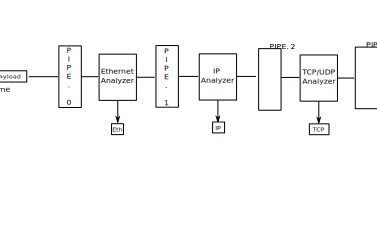
\includegraphics[width=0.95\textwidth]{chapters/pic/ParserTop}
    \caption{HFE~M2 architecture.}
    \label{fig:hfem2Arch}
\end{figure}  

Protocol analyzer uses the \textit{Generic Protocol Parser Interface} (GPPI) for connection between modules. This interface
provides the input information necessary to parse a single protocol header. That is: (1)~current packet data being
transferred at the data bus, (2)~current header offset within the packet and (3)~expected protocol to parse. 
GPPI output information includes (4)~extracted packet header field values, plus the information needed to 
parse the next protocol header: (5)~next header offset
and (6)~type of the next protocol header. More details about the GPPI can be found in \cite{hfem2}.
Brief architecture of each Protocol Analyzer block is shown in Fig.~\ref{fig:protocolArch}. 

\begin{figure}[ht]
    \centering
    \includegraphics[scale=1.25]{chapters/pic/ProtocolAnalyzer}
    \caption{Protocol analyzer architecture.}
    \label{fig:protocolArch}
\end{figure}    

Protocol analyzer architecture contains four block types: (1)~Data Extractors, (2)~Next Protocol Decoder, 
(3)~Length Generator and (4)~Adder. Data Extractors are used to extract packet data from a given offset. 
Data Extractors are configured with two parameters: \textit{Extract Length} and \textit{Extract Offset}. 
The first parameter defines the number of extracted bytes from packet data. The offset of data within the packet is computed as the sum
of current header offset (a value from input GPPI interface) and the Extract Offset parameter.
Note that Data Extractor blocks contain multiplexers which allow to extract data from any byte position. 
These multiplexers can be configured with some additional optimization parameters which  
reduce consumed FPGA resources. We describe these parameters in Sec.~\ref{sec:optimizations}.

Next Protocol Decoder is used to compute the next expected protocol. Its structure fully depends on the protocol header format.
Generally, it is a function converting some extracted packet header bytes into an internal number representing the protocol type.

Length Generator block is used to compute the length of current protocol header, so that it can be added to the Input Offset signal to obtain 
the Output Offset signal, which represents the start offset of the next protocol header.
The added offset value can be a constant or a result of an expression (see the header format specification in previous chapter).

From the perspective of parser generation, we can identify three types of blocks in the Protocol Analyzer structure 
(see Fig.~\ref{fig:protocolArch}): (1)~Static (green color), (2)~Configured (grey color), 
(3)~Fully protocol-specific (blue color). 
The static block is used in every Protocol Analyzer without any change. 
The Protocol Analyzer architecture contains only one static block, which is the adder.
This block is used to compute the next protocol offset from current Input Offset and Length Generator output. 
The second group of blocks is general enough for usage in all Protocol Analyzers, only with different parameters settings. 
The architecture contains several Data Extractor blocks which 
are instantiated (from a hand optimized template) and configured regarding to P4's Header Format specification. 
Blocks marked by blue color are entirely protocol specific, so that every Protocol Analyzer needs custom implementation of them.
This means that Protocol Decoder and Offset Generator must be uniquely generated for each Protocol Analyzer from P4's Header description.

This architecture of Protocol Analyzer is general enough for processing of most L2-L4 protocols. 
For this target block structure, we can generate, configure and connect all described blocks in automatic way from a P4 program. 
Details of this transformation process are discussed in the next section.

\subsection{Transformation from the P4 to Parser Architecture}
\label{sec:parserTransformation}

Transformation algorithm is one of the key problems addressed in this chapter.
As we note in Sec.~\ref{sec:overviewOfHfeM2}, HFE~M2 architecture consists of Protocol Analyzers and pipeline modules which are
connected to form the processing chain. 
The transformation from P4 to parser can be divided into two problems --- (1)~Generating the Protocol Analyzers and 
(2)~Generating the processing chain.
Inputs of the transformation process are P4's Header Format and \textit{Parser Graph Representation}.

We define the \textit{Parser Graph Representation} (PGR) as an acyclic oriented graph which is generated from the P4's Packet Parser definition. 
Each node (or state) represents one packet header and each transition represents the next parsed protocol header. 
Each transition is taken based on the parsed data. Condition of a transition is inferred from the P4's Packet Parser definition.
%Loop edge represents the situation when we want to support more protocols of the same type in protocol stack 
%(like VLAN or MPLS stacking, for example).
Each non-final state contains additional transition to the \textit{Unknown} state. 
This state is not explicitly described in P4 program but it is implicitly required by the parser. 
It represents the situation when no value matches the actual set of transition conditions 
(i.e., we cannot continue in parsing of next protocol header).
Each PGR node also contains a pointer to P4's Header Format definition which is needed during generation of individual Protocol Analyzers.
The PGR representation is built from a P4's Packet Parser definition.
%using the \textit{depth-first search}\,(DFS) algorithm. 
We introduce more details about this structure in the following text. 
An example of this generated representation is in Fig.~\ref{fig:parserGraph}. 
The figure doesn't show transition conditions in order to keep it well arranged.

\begin{figure}[ht]
    \centering
    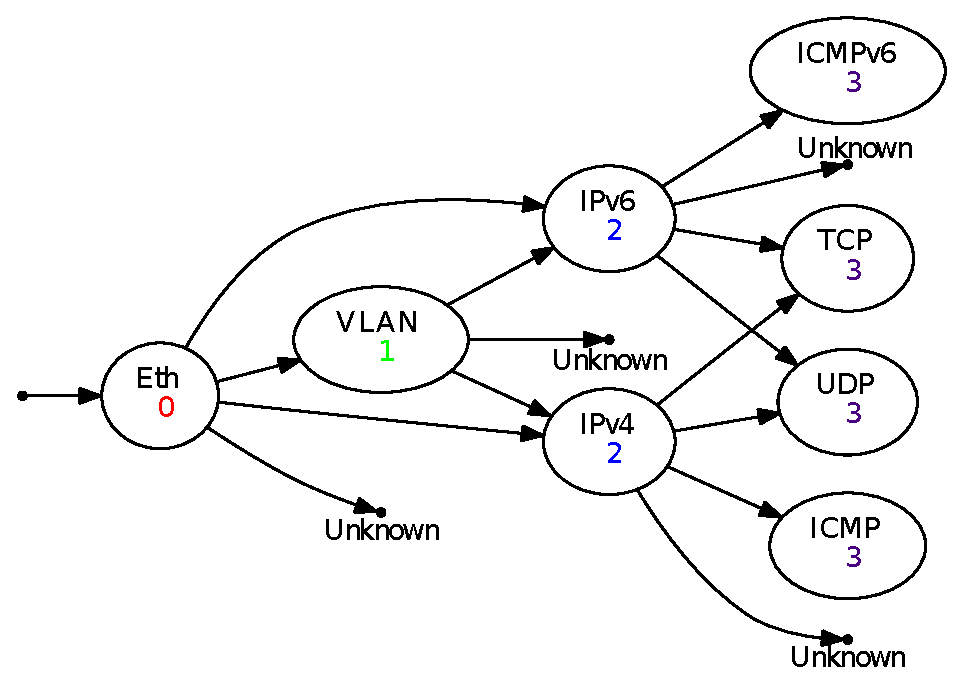
\includegraphics[scale=0.55]{chapters/pic/ParserGraph}
    \caption{Parser Graph Representation; The example supports Ethernet, VLAN, IPv4, IPv6, TCP, UDP, ICMP and ICMPv6.}
    \label{fig:parserGraph}
\end{figure}

As we note in \ref{sec:overviewOfHfeM2}, each Protocol Analyzer consists of three types of blocks (see Fig.~\ref{fig:protocolArch}). 
We now describe the generation of Protocol Analyzer block:
\begin{itemize}
\item The Length Generator block is derived directly from P4's Header Format definition. 
It can be either a constant in the case of constant length header, or a (usually simple) formula in the case of variable length header.
\item The Next Protocol Decoder is also generated from the P4's Packet Parser description. Each transition from the parser state is described
in the P4's \textit{switch} statement by the tuple, including \textit{value} and \textit{next state}. 
Therefore, we can implement Protocol Decoder by a multiplexer which selects the next protocol based on currently parsed values. 
The protocol headers that follow the currently parsed one are found in PGR during the generation.
Data Extractor blocks are parameterizable modules which are used in all Protocol Analyzers without any change, 
only by setting the parameters to match the target protocol. 
There are two parameters for each Data Extractor: Extract Length (number of bytes to be extracted) and 
Extract Offset (byte position of the extracted field, relative to the first byte of protocol header).
\item Extracted Data of Packet Analyzer can be inferred from the Header Format specification because we know the structure of protocol fields 
in the parsed protocol.
Therefore, protocol fields can be extracted from packet data using the list of protocol fields and their sizes. 
\item Adder is a static block common to all Protocol Analyzers. 
\end{itemize}

\begin{algorithm}[t]
    \caption{Recursive algorithm for identification of node levels.}
    \label{alg:longest}
    \SetAlgoLined
    \SetKwFunction{FindNodeLevels}{FindNodeLevels}
    \SetKwProg{myalg}{Function}{}{}
    \myalg{\FindNodeLevels{node, curr\_level}}{
        \KwInput{node = actual node to process}
        \KwInput{curr\_level = actual level of the node}
        \KwResult{Node with updated maximal level}
        \Begin{
            \If {node.fresh == False}
            { return\;}
            \BlankLine
            \tcc{Mark the node as not fresh and update the level}
            node.fresh = False\;
            act\_level = node.get\_level()\;
            \If{act\_level \textless curr\_level}
            { node.set\_level(curr\_level)\;} 
            \BlankLine
            \tcc{For all fresh successors, update the level and call the same function}
            node\_successors = node.get\_next\_states()\;
            \For{next\_node {\normalfont \textbf{in}} node\_successors}
            { \tcc{Don't call the node if the longest path already exists}
                \If{next\_node.get\_level() - node.get\_level() \textless 1}
                {\FindNodeLevels{next\_node,curr\_level+1}\;}
            }   
            \BlankLine
            \tcc{Mark the node as not visited}
            node.fresh = True\;
            \KwRet\;}{}}
\end{algorithm}

When generating the Next Protocol Decoder, Length Generator blocks 
and Extracted Data outputs, Data Extractors are instantiated and parametrized as needed.
Both parameters (Extract Length and Extract Offset) are directly derived from the P4 description of translated program.

Previous text introduces the automatic generation of Protocol Analyzer from P4 source code. 
The following text provides details about the automatic generation of processing chain.
The key problem is to identify a place for insertion of each Protocol Analyzer in the chain. 
Therefore, the planning algorithm has to fulfill following requirements:
\begin{enumerate}
    \item The planned structure of modules has to form a pipeline (due to the parser architecture).
    \item Protocol at the end of each transition has to be processed after the protocol at the beginning of that transition.
    \item The ordering of Protocol Analyzers has to be carefully planned because the architecture doesn't allow feedback loops.
    Planned modules have to form a totally ordered set such that it contains all possible ways through the PGR (node skipping is allowed).
    \item The ordered set can be found using the \textit{depth-first search}\,(DFS) algorithm where the output is a \textit{level} of 
    each node (i.e., the latest possible use of a protocol in pipeline).
   %The \textit{level} is used during generation of pipeline because it represents the latest possible use of a protocol in generated structure.
\end{enumerate}

\begin{algorithm}[t]
    \caption{Brief transformation algorithm from P4 to parser.}
    \SetAlgoLined
    \label{alg:transformationParserAlg}
    \SetKwFunction{TransformationToParser}{TransformationToParser} 
    \SetKwProg{myproc}{Procedure}{}{}
    \myproc{\TransformationToParser{prog}}{
        \KwInput{prog = P4 Program}
        \KwResult{VHDL code of the parser}
        \Begin{
            \tcc{1) Identify the Parser Graph Representation}
            parser\_graph = \texttt{GetParserGraphRepresentation}(\textit{prog})\;
            \BlankLine
            \tcc{2) Mark all nodes as Fresh. After that, traverse through the graph and identify level of each node}
            \texttt{MarkFresh}(\textit{parser\_graph})\;
            \texttt{FindNodeLevels}(\textit{parser\_graph.root,0})\;
            \BlankLine
            \tcc{3) Generate Protocol Analyzers and processing chain}
            \texttt{GenerateProcessingChain}(\textit{parser\_graph})\;
        }
    }
\end{algorithm}

\begin{figure}[b]
    \centering
    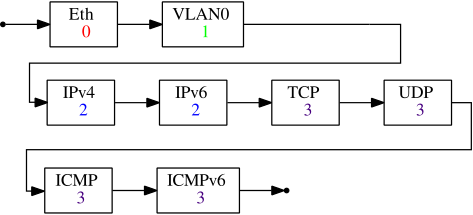
\includegraphics[scale=0.67]{chapters/pic/ParserPipeline}
    \caption{Generated processing chain; Pipeline modules are omitted for brevity.}
    \label{fig:parserPipeline}
\end{figure}

The generator of processing chain uses a PGR as an input. 
Its task is to identify the longest paths from root to each node in PGR (i.e., \textit{level} of each node). 
If we have several nodes on the same \textit{level}, we connect Protocol Analyzers in series with arbitrary ordering.
While same-\textit{level} analyzers could be connected in parallel, the serial approach allows us to keep the homogeneous structure of processing chain.
The longest paths in a PGR is found using the Alg.~\ref{alg:longest}. 
The algorithm recursively traverses and identifies node \textit{levels} in inspected graph.
The result of this algorithm is shown in Fig.~\ref{fig:parserGraph}, where each node contains a number which represents the length of the longest path 
from root. 

Finally, we introduce the Alg.~\ref{alg:transformationParserAlg} which is used for generation of complete 
parser architecture from a P4 description.
We implemented this transformation algorithm in Python language with usage of P4-HLIR \cite{p4hlir} project. 
The result of Alg.~\ref{alg:transformationParserAlg} can be seen in Fig.~\ref{fig:parserPipeline} which represents 
the processing chain generated from the PGR in Fig.~\ref{fig:parserGraph}. 
The Fig.~\ref{fig:parserPipeline} doesn't contain any pipeline modules for brevity, but the real firmware implementation contains a pipeline 
module between each two adjacent Protocol Analyzers. 
This figure also shows the situation when two or more different nodes are situated on the same level. 
Such nodes are connected in series and their relative position doesn't matter.
The only rule is to keep them together (i.e., the generator connects modules which belong to the same level in series). 


\subsection{Optimizations}
\label{sec:optimizations}

The original hand-written HFE~M2 parser supports several optimizations which save a significant amount of chip resources. 
Therefore, we have decided to support some of these optimizations in our generator as well.

The first optimization is related to Protocol Analyzer's GPPI interface. The key idea is to optimize the width of the offset bus which is used for 
signalization of protocol header start position (Input Offset and Output Offset signals). 
In another words, Input Offset and Output Offset signals are \emph{pointers} into the packet.
Since the protocol stack is being analyzed in sequential manner within the packet, the width of offset bus can increase in sequential 
manner too --- it is unnecessary to implement 
all logic (adders, etc.) at full data width, especially in early pipeline stages. 
The bus width parameter is inferred from maximal protocol header lengths
during translation. The bus width at each level is computed as a binary logarithm of the sum of all preceding protocol header lengths.
Narrower offset bus leads to smaller modules for computation of next header offset and other required values.
Therefore, we save chip resources and possibly raise the working frequency.

\begin{figure}[b]
    \centering
    \includegraphics[scale=0.91]{chapters/pic/MuxOpt}
    \caption{The example of data extraction multiplexer: full (a), optimized (b).}
    \label{fig:muxOpt}
\end{figure}

The second optimization is related to data extraction which is performed by multiplexers within Data Extractor blocks. 
Generally, each Data Extractor is able to extract data 
from any byte position in the packet bus data word. The multiplexer is controlled by current data bus offset and offset of the 
desired field within the header. However, given the fact that the packet header may start only at certain positions on the data bus, current 
offset can contain only values with the corresponding resolution. 
This resolution is computed from P4's Header Format and Packet Parser definition. 
Using these two specifications, we identify the Offset List which contains all possible starting positions of each analyzed header in 
the processing chain. 
This knowledge is built from a protocol header length and relations between protocol headers by simulation of data transfer on data bus.
Computed lists are used for identification of required multiplexer's parameters. 
By making Data Extractors less general, we simplify the structure of each extraction multiplexer and save available chip resources. 
An example of this optimization is shown in Fig.~\ref{fig:muxOpt}. 

The multiplexer parameters can be computed from Offset List $\textbf{b}=(b_0,b_1,\dots,b_n)$ 
using the Alg.~\ref{alg:muxParamsComp} where each Offset List element represent one starting protocol offset. 
The proposed algorithm is based on observation that each offset can be expressed in the form $k*2^n + q$ where:
\begin{itemize}
    \item  $k \in {\mathbb N_0}$ represents the index of multiplexer block,
    \item  $2^n, n \in {\mathbb N_0}$ represents the size of multiplexer block,
    \item  $q, 0 \leq q < 2^n, q \in {\mathbb N_0}$ represents the offset in multiplexer block.
\end{itemize}

In other words, we want to find a common granularity for all starting offsets which are represented by a multiplexer block 
size and internal offset.

\begin{algorithm}[!b]
    \caption{Computation of multiplexer parameters.}
    \SetAlgoLined
    \label{alg:muxParamsComp}
    \KwInput{Offset List: ${\mathbf b} = (b_0, b_1, \dots , b_n), n \in {\mathbb N_0} $}
    \KwResult{Computed parameters: $n \in {\mathbb N_0}, q \in {\mathbb N_0}$}
            \BlankLine
    \tcc{Starting values (extraction from each byte position)}
    $n = 0$\;
    $q = 0$\;
    $div = 2$\;
    \BlankLine
    \While{True}{
        \tcc{Compute the reminder for each element in ${\mathbf {tmp}}$ vector}
        \For{$b_i$ \textbf{in} ${\mathbf b}$}{
            $tmp_i$ = $b_i\ mod\ div$\; 
        }
        \tcc{Check reminders in ${\mathbf {tmp}}$ vector}
        \eIf{$tmp_i == tmp_0,\ \forall tmp_i \in {\mathbf {tmp}} $} {
            \tcc{All reminders are identical. Remember the actual result and try next iteration.}
            $n = \lceil log_2(div) \rceil$\;
            $q = tmp_0$\;
            $div = 2*div$\;
        }{
            \tcc{All elements are not same. Stop the algorithm.}
            break\;
        }
    }
    \BlankLine
    \Return $n,q$
\end{algorithm}

There is also a place for optimizations of P4 program which cannot be automatically generated. 
Instead, it is required to optimize the program during design time.
The generator can then benefit from more efficient input, which results in better design in terms of latency and consumed resources. 
In this text, we introduce one such optimization 
of P4 program which leads to less Protocol Analyzer blocks being generated.
The idea is to merge protocol headers that are compatible in terms of extracted protocol header fields.
As an example, we want to extract source and destination ports of TCP and UDP protocols because their structure is similar. 
Therefore, we create a new custom protocol header which describes export of interesting fields.  
We don't have to worry about incomplete protocol header specification because our replaced protocol headers are 
leaves of the PGR (see Fig.~\ref{fig:parserGraph}), so that there is no further processing after this merged header.
We define the new protocol header like this:
\begin{Verbatim}[fontsize=\small]
header tcp_udp_t {
   fields {
      src_port : 16; // width in bits
      dst_port : 16;
   }
}
\end{Verbatim}

\subsection{Time Complexity of the Transformation}
\label{sec:parserTimeComplexity}

Time complexity of the proposed transformation Alg.~\ref{alg:transformationParserAlg} consists of following components (consider situation
without computation of multiplexer parameters):
\begin{enumerate}
    \item \texttt{GetParserGraphRepresentation}'s time complexity is equal to $\mathcal{O}(V+E)$ (DFS algorithm), where $V$ is the number of nodes and 
$E$ is the number of edges. Our transformation algorithm requires PGR with no cycles.
In general, maximal number of edges in acyclic graph is equal to $\frac{n}{2}*(n-1)$ where $n$ is the number of Protocol Analyzers 
(i.e., nodes of our graph). Total time complexity of DFS is $\mathcal{O}(n+\frac{n}{2}*(n-1)) \sim \mathcal{O}(n^2)$.
    \item \texttt{FindLongestPaths}'s time complexity is equal to $\mathcal{O}(n^2)$ (DFS algorithm), where $n$ is the number of Protocol Analyzers.
    \item \texttt{MarkFresh}'s time complexity is equal to $\mathcal{O}(n)$, where $n$ is a number of protocols (i.e., nodes of PGR).
    \item \texttt{GenerateProcessingChain}'s time complexity is equal to $\mathcal{O}(n)$ because generated processing chain contains $n$ 
    Protocol Analyzers. 
\end{enumerate}

Total time complexity of the transformation (without computation of multiplexer parameters) is 
$\mathcal{O}(n^2)+\mathcal{O}(n^2)+\mathcal{O}(n)+\mathcal{O}(n)=\mathcal{O}(2*n^2)+\mathcal{O}(2*n) \sim \mathcal{O}(n^2)$.

The list of protocol offsets is constructed using the DFS algorithm. Therefore, the time complexity is $\mathcal{O}(\frac{n}{2}*(n-1))$
where $n$ is the number of Protocol Analyzers. Notice that the length of Protocol Analyzers's offset list depends on complexity of PGR.

Computation of multiplexer parameters cannot use more than $\mathcal{O}(log_2(\max({\mathbf b})))$ iterations 
(i.e., the number of binary digits of maximal element in the vector) where the algorithm
requires $\mathcal{O}(\text{len}(\mathbf{b}))$ time for initialization of $tmp$ vector and $\mathcal{O}(\text{len}(\mathbf b))$ for check of
all reminders in $tmp$ vector. The total time complexity of the algorithm is 
$\mathcal{O}(2*\text{len}(\mathbf b)*log_2(\max({\mathbf b}))) = 
\mathcal{O}(\text{len}(\mathbf b)*log_2(\max({\mathbf b})^2))$ where
$\mathbf b$ is a merged list of protocol offsets of all Protocol Analyzers.

\section{Deparser Architecture}
\label{sec:deparserArch}
% Sepsat zakladni architekturu deparseru, ta se muze vzit z MICPRO
% Pridat zakladni info o propustnosti (udelat analyzu)
The deparser module is used to assemble packets back from modified protocol headers. 
The architecture of our deparser module (published in \cite{2016pesw,2016h2rc-p4,2016MicproP4}) is similar to HFE~M2 \cite{hfem2}. 
It consists of two modules --- Protocol Appenders and pipelines. 
Protocol Appender effectively inserts a protocol header before payload (i.e., it merges protocol header and payload). 
There is an optional pipeline block between each two Protocol Appenders. This pipeline block has the same 
reason as in the case of parser pipelines. They are also used for tuning of final frequency, latency and chip area. All modules
are connected to the processing chain which represents the supported protocol stack. 
Brief architecture is 
shown in Fig.~\ref{fig:deparserArch}. The figure also introduces the main idea of deparser's architecture --- all modules are connected
in reverse order (from upper protocol layers to lower protocol layers), where each Protocol Appender inserts the header at zero offset. 
Generally, there are two approaches for stacking of appending units --- botom-to-up and up-to-bottom. 

\begin{figure}[ht]
    \centering
    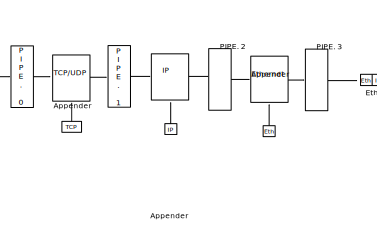
\includegraphics[width=0.95\textwidth]{chapters/pic/DeparserTop}
    \caption{Deparser architecture.}
    \label{fig:deparserArch}
\end{figure}

The bottom-to-up approach is similar to the solution of parser (i.e., insertion from lower protocol layers to upper protocol layers). 
This approach is natural for the implementation in a software program which typically fills the packet memory in sequential manner.
However, this is not suitable for hardware implementation because each Protocol Appender would have to support multiple \emph{insertion offsets} 
(the set of supported insertion offsets depends on previously inserted headers). 
This leads to more complex shifting logic which consumes more FPGA resources.

The up-to-bottom approach makes the assembling process easier because 
the appended header is inserted always at the beginning of the packet (i.e., at zero offset).
To make that possible, the incoming data of unfinished packets must be shifted to make space for the new header.
The incoming data are fixed to zero offset. 
Therefore, the shifting logic is insensitive to previous Protocol Appenders and the complexity of shifting logic depends only on the current protocol.

The Protocol Appender uses a generic interface for connection between modules. This interface provides the input information 
necessary to assemble a single protocol header. That is: (1)~current protocol header fields to be inserted, (2)~current (unfinished) packet 
to insert the header into and  (3)~header insertion vector where each Protocol Appender observes one bit position. 
This observed bit enables or disables the header insertion. 
The output information includes (4)~merged data and (5)~unmodified header insertion vector.
Notice that incoming unfinished packet always starts on the first byte of data bus.

\begin{figure}[ht]
    \centering
    \includegraphics[scale=1.27]{chapters/pic/ProtocolAppender}
    \caption{Protocol Appender architecture.}
    \label{fig:protocolAppender}
\end{figure}

Architecture of Protocol Appender contains three block types: (1)~Data Width Transform, (2)~Header Merger and (3)~Enable logic.
The Data Width Transform unit is used to transform the header from its native data width (w1), given by the sum of its fields, to the width of 
the main data pipeline (w2).
This transformation leads to a simpler data merging process. The Enable logic is a simple detector which observes predefined 
bit position in header insertion vector. The observed bit enables or disables the header insertion. 
The width of this input vector equals to the number of used Protocol Appenders in the processing chain. 

The Header Merger consumes three inputs --- transformed header data, payload and enable signal. 
It is divided into three
sub-blocks. The first, Data Shifter, is used to make a free space in the incoming unfinished packet data.
It moves the data behind the free space where the current packet header is to be inserted
in Data merger sub-block. The Data merger sub-block implements an effective merging logic where both inputs (header and payload) 
are masked by logical \textit{and} operation and merged by logical \textit{or} operation. 
The whole process of merging is controlled by the Finite State Machine (FSM) which controls the logical operations. If no header is 
inserted in actual Protocol Appender stage, the FSM disables header interface (i.e., \textit{and} operation with data and zero vector) and
the payload is transferred unchanged (i.e., logical \textit{or} between zero vector and incoming payload is performed).
 
There is also a possible optimization which can be inferred from the property of incoming protocol. All protocols can be
divided into two groups --- protocols with static and dynamic header length. In the first group, we have to support two shifting
offsets --- zero offset (i.e., no change of payload structure) and static offset (i.e., offset of shifted payload by a constant). 
This kind of offset can be computed with equation \ref{eq:offset} where $l$ is the length of inserted header in bytes and $w$ 
is the width of payload bus in bytes. In other words: payload is shifted to the next available byte position behind the inserted header. 
The proposed equation can be used if inserted header doesn't occupy the whole output bus width 
(the result of the equation \ref{eq:offset} differs from zero). 
If header occupies the output bus (the result equals to zero), 
we have to move the payload insertion to the next bus cycle with zero offset value 
(i.e., we don't need to modify the offset of incoming payload).
The example of header insertion is demonstrated in Fig.~\ref{fig:protocol-appender-princip}.

\begin{equation}
\textrm{offset} \equiv (l+1) \;(\bmod\; w)
\label{eq:offset}
\end{equation}

The case with dynamic protocol length is more complex, because we need to support more shifting offsets. The reason
for this is straightforward --- we don't know the exact length of the protocol header during the compile time. 
Therefore, we have to support more complex shifting logic based on granularity of inserted protocol.
The shifting multiplexer can be also optimized in similar way like data extraction multiplexers in parser.

\begin{figure}[ht]
    \centering
    \includegraphics[scale=0.45]{chapters/pic/ProtocolAppenderPrincip}
    \caption{The example of header insertion in Protocol Appender.}
    \label{fig:protocol-appender-princip}
\end{figure}

\subsection{Transformation from the P4 to Deparser Architecture}
\label{sec:deparserTransfAlg}

The transformation algorithm from P4 to deparser architecture is quite similar to generation of parser. We can reuse
the PGR and \textit{depth-first-search}\,(DFS) algorithm for identification of node levels. 
After the identification, we reverse the order of Protocol Appender modules.
The transformation algorithm can be described using the Alg.~\ref{alg:transformationDeparserAlg}

\begin{algorithm}[ht]
    \caption{Brief transformation algorithm from P4 to deparser.}
    \SetAlgoLined
    \label{alg:transformationDeparserAlg}
    \SetKwFunction{TransformationToDeparser}{TransformationToDeparser} 
    \SetKwProg{myproc}{Procedure}{}{}
    \myproc{\TransformationToDeparser{prog}}{
    \KwInput{prog = P4 Program}
    \KwResult{VHDL code of the deparser}
        \Begin{
            \tcc{1) Identify the Parser Graph Representation}
            parser\_graph = \texttt{GetParserGraphRepresentation}(\textit{prog})\;
            \BlankLine
            \tcc{2) Mark all nodes as Fresh. After that, traverse through the graph and identify level of each node}
            \texttt{MarkFresh}(\textit{parser\_graph})\;
            \texttt{FindNodeLevels}(\textit{parser\_graph.root,0})\;
            \BlankLine
            \tcc{3) Reverse the order of PGR nodes and generate the processing chain}
            deparser\_graph = \texttt{ReverseNodeLevels}(\textit{parser\_graph})\;
            \texttt{GenerateDeparsingChain}(\textit{deparser\_graph})\;
        }
    }
\end{algorithm}

The result of the proposed algorithm is a processing chain similar to the example in Fig.~\ref{fig:parserPipeline}.
The only difference is the reversed order of all modules. 

\subsection{Time Complexity of the Transformation}
The time complexity of the Alg.~\ref{alg:transformationDeparserAlg} is similar to the Alg.~\ref{alg:transformationParserAlg}.
However, there are two important differences. The first difference is related to \texttt{GenerateDeparsingChain}. 
This function contains computation of multiplexer parameters for appending logic. The logic needs to support just offsets of appended protocol. 
Therefore, the number of supported offsets is typically smaller than the list of supported offsets in the last Protocol Analyzer of 
more complex PGR. 
The second difference is related to the \texttt{ReverseNodeLevels}. 
This function is used for generation of deparser's structure in $\mathcal{O}(n)$ time where $n$ is the number of Protocol Appenders. 
Therefore, the time complexity of the Alg.~\ref{alg:transformationDeparserAlg} is
$\mathcal{O}(n^2)+\mathcal{O}(n^2)+\mathcal{O}(n)+\mathcal{O}(n)+\mathcal{O}(n)=\mathcal{O}(2*n^2)+\mathcal{O}(3*n) \sim \mathcal{O}(n^2)$.

\section{Parser-Deparser Experiments}
% Sepsat tady analyzu jaka bude minimalni mozna propustnost, vyjde ze to neda maximum 100 Giga, ale
% mame obecne reseni, ktere se da pouzit i v jinych resenich (porad je to obecne). Vysledky mereni
% v FPGA.
In this section, we introduce results for parser and deparser because both modules are usable standalone.
We have tested properties of generated parsers with two different protocol stacks:
\begin{itemize}
    \item \textbf{simple L2} - Ethernet, IPv4/IPv6 (with 2$\times$extension headers), TCP/UDP, \\ ICMP/ICMPv6
    \item \textbf{full} - Ethernet, 2$\times$VLAN, 2$\times$MPLS, IPv4/IPv6 (with 2$\times$extension headers), \\ TCP/UDP, ICMP/ICMPv6
\end{itemize}

For each protocol stack, we compare the manually optimized HFE~M2 parser and the generated parser with all optimizations enabled. The 
deparser isn't compared to a hand optimized version because this architecture was tailored to needs of 
automatic generation and there is no other hardware based deparser available.
All tested designs implement both engines without any additional logic like outputs FIFOs for parsed data, cleanup logic, etc. 
We choose this approach because the additional logic typically depends on the character of implemented application. 
We use the Slice Logic (number of used LUTs plus FlipFlops) as a metric of resource utilization because these parts are the most utilized in 
most FPGA designs.

We provide results after synthesis for the Xilinx Virtex-7 XCVH580T FPGA using the Xilinx Vivado 2015.1 design tool. 
All designs were synthesized with different settings of data width and presence of pipeline modules. 
These settings, together with the resulting frequency, latency and resource usage, generate a large space of
possible solutions for each P4 program. 
These solutions were searched for Pareto set which allows us to pick the best-fitting solution for an application.

\subsection{Results for the Parser}
\label{sec:exprParser}

In each \textbf{hand optimized} design test case, we
use two different data widths: 256 and 512 bits. For each data width, every possible placement of pipelines was tested: $2^{9}$ possible combinations 
in the case of the full protocol stack and $2^{5}$ combinations in the case of simple L2 protocol stack (because there are 9 and 5 configurable pipeline stages). 

In each \textbf{generated} parser test case, we use two different data widths: 256 and 512 bits. 
For each simple L2 parser, every possible placement of pipelines was tested: $2^{10}$ possible combinations. 
In the case of full parser, there are $2^{14}$ different configurations. We have randomly selected 20\% of all possible solutions.
This approach allows us to briefly inspect properties of generated processing chain in a reasonable compile time.

We provide two graphs with Pareto sets: one showing Pareto sets optimized for throughput and chip area without any regard to latency, 
and second optimized for throughput and latency without any regard to FPGA resources. 
Before the graphs, we introduce results for optimizations which are described in 
Sec.~\ref{sec:optimizations} because they have an influence on latency and used resources. We define the following notation:
\begin{itemize}
    \item \textbf{No optimizations (O0)} - no optimizations are used.
    \item \textbf{Offset optimization (O1)} - optimization of the offset width.
    \item \textbf{Offset + multiplexer optimization (O2)} - offset and multiplexer optimizations.
    \item \textbf{Optimized P4 program (O3)} - O0 version with effectively written P4 program (manual optimization).
    \item \textbf{All optimizations (O4)} - all proposed optimizations are used.
\end{itemize}

Resource utilization (values in parentheses represent the percentual usage of available FPGA's resources) and latency for parsers 
generated with different optimizations are shown in Tab.~\ref{tab:optMethod}. The table shows the influence of proposed optimizations on
similar hardware configurations with throughput around 100\,Gbps. 

\begin{table}[ht]
    \centering
    \begin{tabular}{|c||c|c|c|c|c|}
        % Header
        \hline
        \T{\textbf{Opt.}} &
        \T{\textbf{Pipes}} &
        \T{\textbf{Latency [ns]}}   & 
        \T{\textbf{Thr. [Gbps]}}  & 
        \T{\textbf{Slice LUT [-]}} & 
        \T{\textbf{Slice Reg [-]}} \\
        \hline\hline
            O0  &    8      &        39.8        &   102.7     &   25335\,(6.98\%)          &   5055\,(0.69\%)           \\ 
            O1  &    14     &        75.3        &   101.9     &   21477\,(5.91\%)          &   8930\,(1.23\%)           \\ 
            O2  &    8      &        46.1        &   100.0     &   10103\,(2.78\%)          &   5537\,(0.76\%)           \\
            O3  &    9      &       44.5         &   115.1     &   14270\,(3.93\%)          &   5427\,(0.74\%)           \\  
            O4  &    7      &       40.7         &   100.7     &   8314\,(2.29\%)           &   4795\,(0.66\%)           \\
        \hline
    \end{tabular}
    \caption{Comparison of different optimization methods with resource consumption for the Xilinx Virtex-7 XCVH580T FPGA.}
    \label{tab:optMethod}
\end{table} 

For all the following results we use O2 optimization, since O3 and O4 require manual modifications to the original P4 program.
We consider this kind of optimization to be highly non-standard.

For comparison of the achieved Pareto set results for different protocol stacks, we provide graphs in Fig.~\ref{fig:hfeParetoLut} 
(throughput and FPGA resources) and Fig.~\ref{fig:hfeParetoLat} (throughput and latency).
The Pareto sets show the best achievable solutions for our parsers. From these figures, we can see that supported protocol stack can significantly 
change parameters of the parser in terms of FPGA resources and latency. 
We can also see that P4 based parsers are approximately two times worse than hand-written parsers in terms of latency and consumed resources. 

\begin{figure}[b]
    \centering
    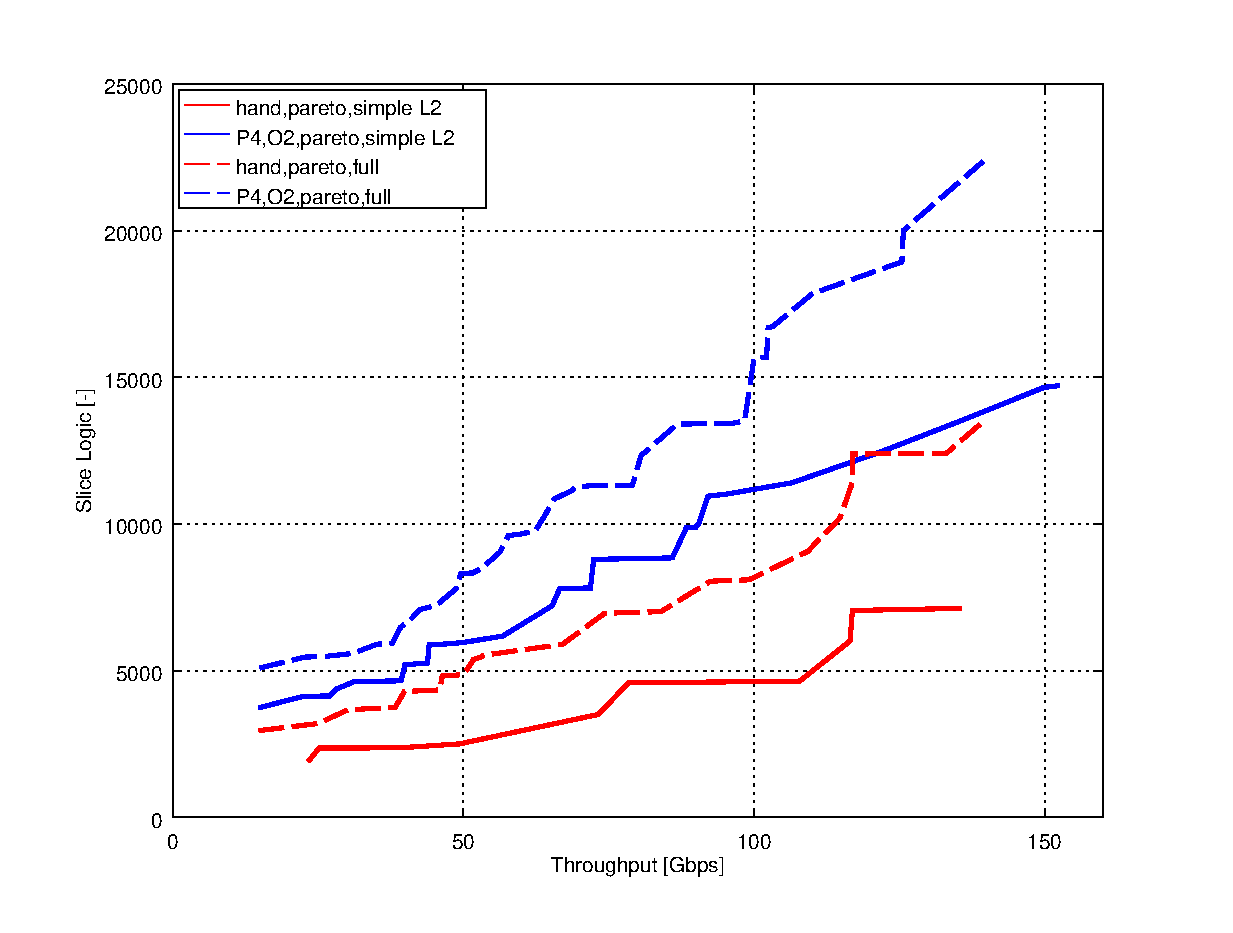
\includegraphics[scale=0.61]{chapters/pic/graphs/hfe/1_thrslice_logic_pareto}
    \caption{Parser - Comparison of the FPGA resource utilization versus throughput Pareto sets for the tested protocol stacks.}
    \label{fig:hfeParetoLut}
\end{figure}

\begin{figure}
    \centering
    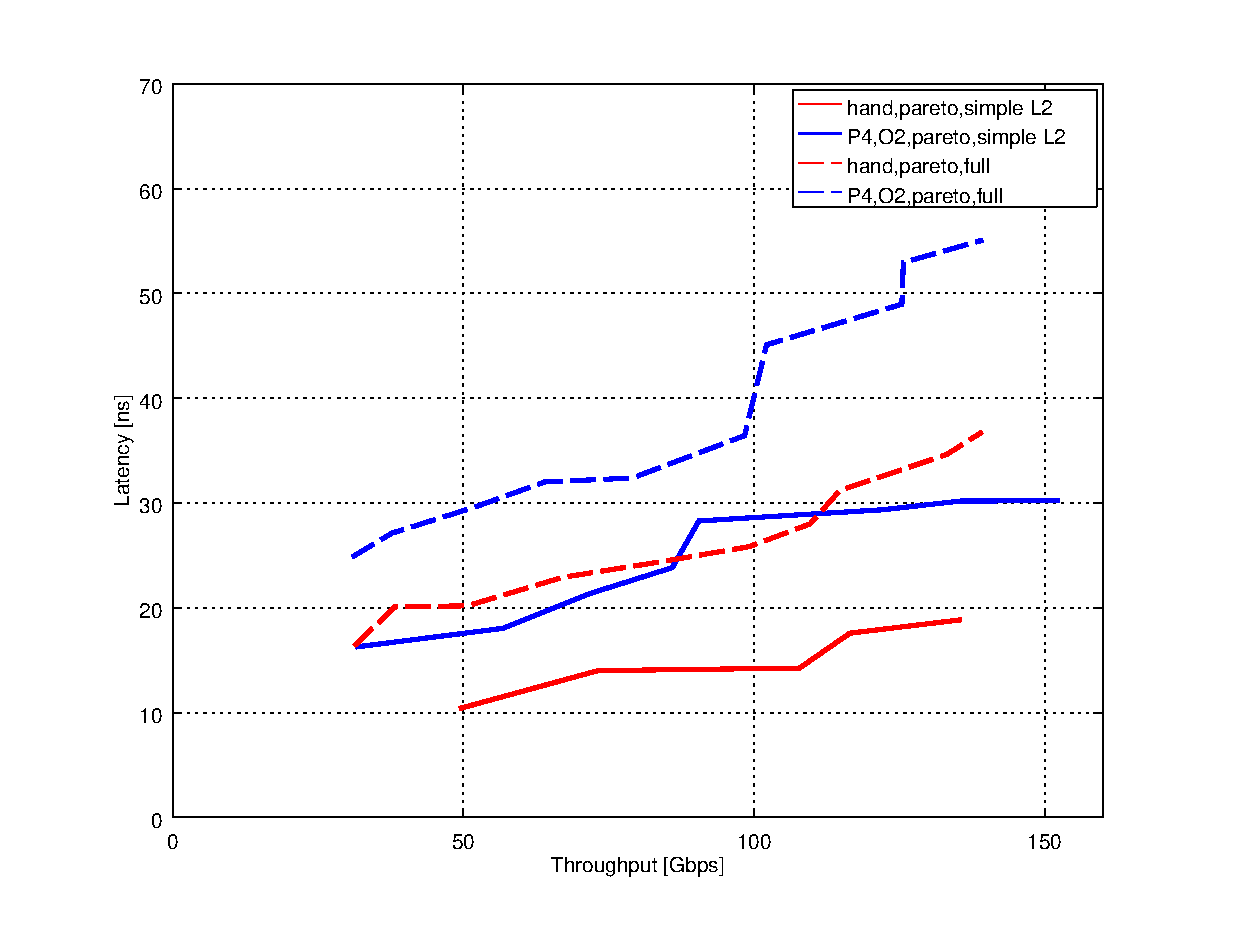
\includegraphics[scale=0.61]{chapters/pic/graphs/hfe/2_thrlat_pareto}
    \caption{Parser - Comparison of the latency versus throughput Pareto sets for the tested protocol stacks.}
    \label{fig:hfeParetoLat}
\end{figure}

\begin{figure}
    \centering
    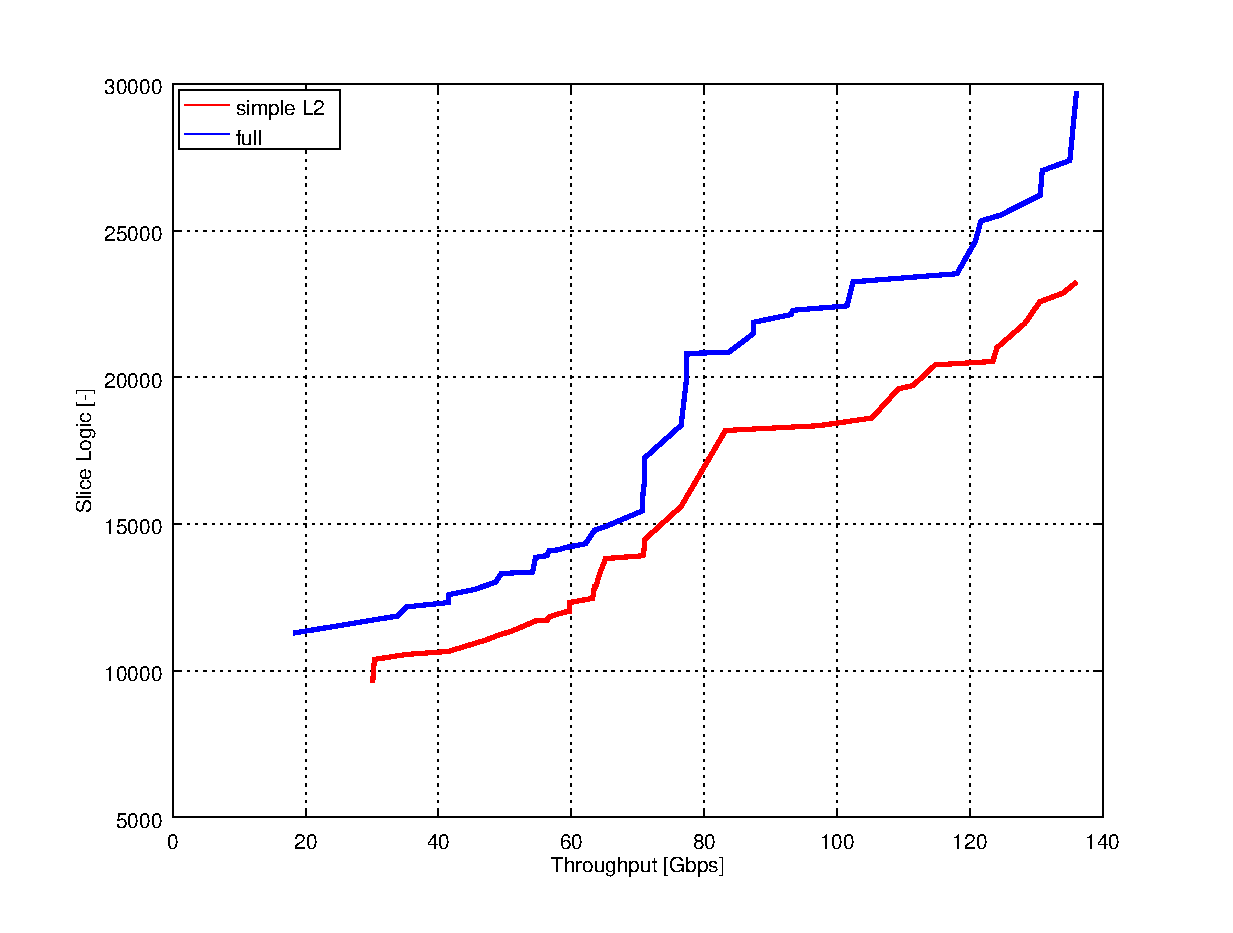
\includegraphics[scale=0.61]{chapters/pic/graphs/deparser/1_thr_slice_logic_pareto}
    \caption{Deparser - Comparison of the FPGA resource utilization versus throughput Pareto sets for the tested protocol stacks.}
    \label{fig:deparserParetoLut}
\end{figure}

\begin{figure}
    \centering
    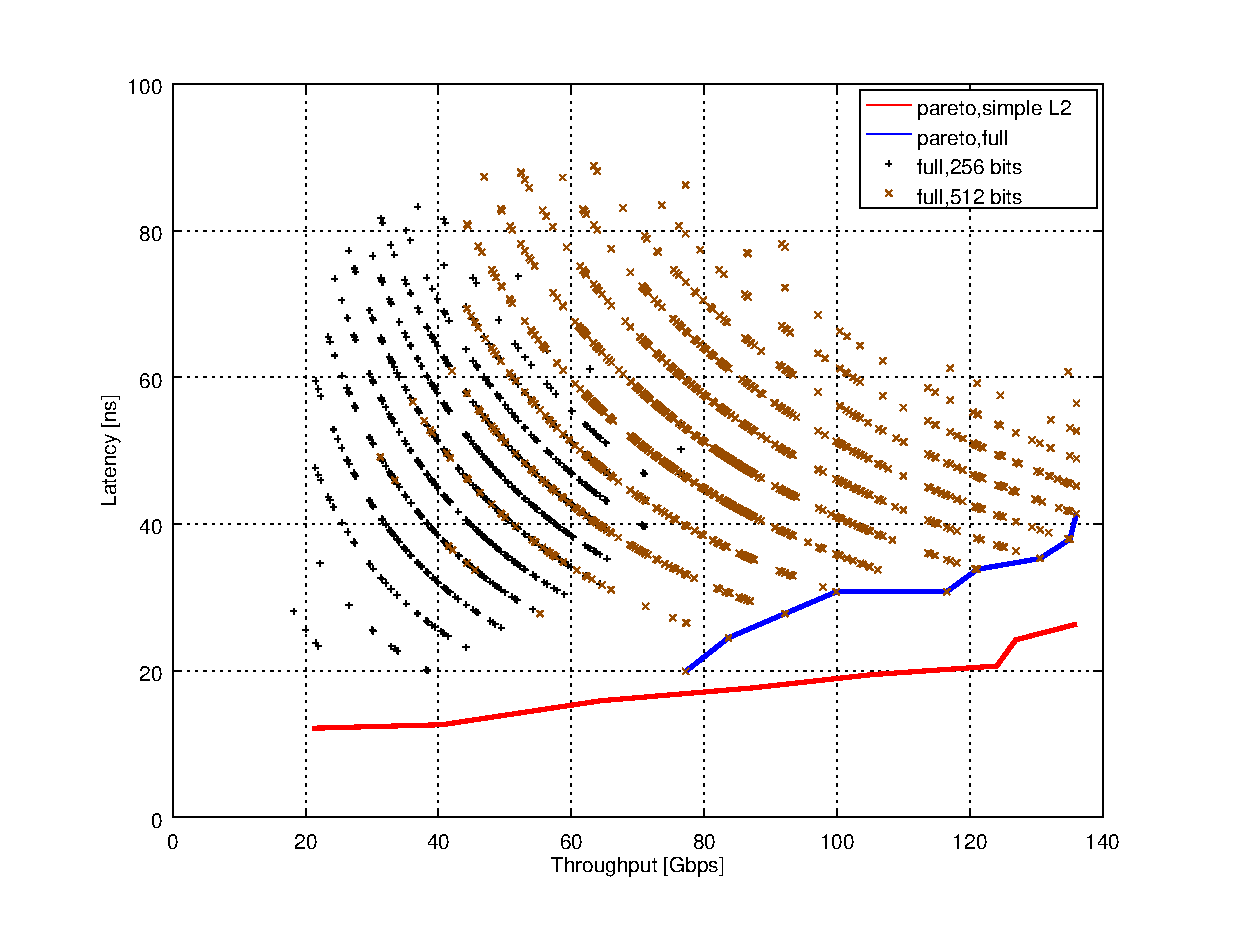
\includegraphics[scale=0.61]{chapters/pic/graphs/deparser/3_thr_latency_deparser.eps}
    \caption{Deparser - Comparison of the latency versus throughput Pareto sets for the tested protocol stacks.}
    \label{fig:deparserParetoLatency}
\end{figure}

\subsection{Results for Deparser}
\label{sec:exprDeparser}

This section introduces results for the deparser module which is used for composition of output packet. We provide graph in
Fig.~\ref{fig:deparserParetoLut} which introduces Pareto sets optimized for throughput and chip area. The graph also 
shows that consumed resources are higher compared to parser with the same throughput. The reason for this is the fact that
each Protocol Appender contains payload shifting logic which consumes more resources than Data Extractor units in parser.
The second graph, Fig.~\ref{fig:deparserParetoLatency}, introduces Pareto sets optimized for throughput and latency. 

The experiment data were measured in the same way like experiments for \textbf{generated} parsers test cases. 
The generated test cases were chosen because we don't have any hand-optimized version of deparser which supports given protocol stacks 
(the architecture of deparser was developed with respect to automatic generation of target architecture). 
Pareto set for latency of full protocol stack starts approximately from 78\,Gbps (see Fig.~\ref{fig:deparserParetoLatency}). 
We provide additional information for illustration of all measured data where each point represents a result for a specific 
configuration of deparser's pipeline.

\subsection{Parser-Deparser Throughput}
\label{sec:exprParserDeparserThroughput}
This section introduces the throughput analysis of Parser-Deparser blocks for the full protocol stack (see Sec.~\ref{sec:exprParser} for details). 
Two use cases will be introduced --- No modification and VLAN tagging.
The first, No modification, represents the raw throughput of both blocks where no changes are performed in parsed headers. 
The second, VLAN tagging, represents the throughput of the generated device during insertion of VLAN header. 
Both engines were generated and synthesized for COMBO-100G card \cite{combo-100g} using the Xilinx Vivado 2015.4 design tool. 
The proposed device is equipped with the Xilinx Virtex-7 XCVH580T FPGA and is capable to process traffic up to 100\,Gbps. All implemented
designs were running at speed of 220\,MHz. We provide two graphs: one showing the percentage throughput of 100\,Gbps Ethernet line and 
second showing the number of mega packets per second (Mpps).

\begin{figure}
    \centering
    \begin{subfigure}[b]{0.8\textwidth}
        \includegraphics[width=\textwidth]{chapters/pic/graphs/parser-deparser/full-plain/throughput.eps}
        \caption{Percentage of maximum throughput.}
        \label{fig:bitThroughputPlain}
    \end{subfigure}
    ~
    \begin{subfigure}[b]{0.8\textwidth}
        \includegraphics[width=\textwidth]{chapters/pic/graphs/parser-deparser/full-plain/mpps-throughput.eps}
        \caption{Packet rate.}
        \label{fig:packetThroughputPlain}
    \end{subfigure}
    
    \caption{Throughput of generated Parser-Deparser device for the No modification use case.}
    \label{fig:noModThroughput}
\end{figure}

\begin{figure}
    \centering
    \begin{subfigure}[b]{0.8\textwidth}
        \includegraphics[width=\textwidth]{chapters/pic/graphs/parser-deparser/full-vlan/throughput.eps}
        \caption{Percentage of maximum throughput.}
        \label{fig:bitThroughputVlan}
    \end{subfigure}
    ~
    \begin{subfigure}[b]{0.8\textwidth}
        \includegraphics[width=\textwidth]{chapters/pic/graphs/parser-deparser/full-vlan/mpps-throughput.eps}
        \caption{Packet rate.}
        \label{fig:packetThroughputVlan}
    \end{subfigure}
    
    \caption{Throughput of generated Parser-Deparser device for the VLAN tagging use case.}
    \label{fig:vlanThroughput}
\end{figure}

The Fig.~\ref{fig:noModThroughput} introduces results of raw throughput (no header modification or insertion was performed). 
We see that generated device is capable to process data at speed of 100\,Gbps. 
However, there are some packet lengths where the throughput falls below 100\,Gbps. 
This decrease of throughput is caused by ineffective usage of available output data bus in deparser.
The most complicated situations occurs on short Ethernet frames. 
We demonstrate this problem on 512 bits wide data bus during transfer of 69 bytes (start of the frame is aligned to the first byte of data bus). 
In this situation, we need to use two bus cycles during which we transfer 69 bytes of Ethernet frame. 
Unfortunately, we are wasting available capacity (i.e., we use 69 bytes from 128 bytes available). 
The case gets less significant with longer Ethernet frames because the data bus is used for longer time and we need to reach smaller packet rate. 
Therefore, minimal throughput of aligned transfer on given packet length can be roughly computed using the equation \ref{eq:thrEq} 
where $dw$ is width of data bus, $freq$ is working frequency, $pkt\_len$ is length of a packet in bytes and $min\_cycles$ is the required 
number of bus cycles for transfer of the packet.

The situation for the VLAN tagging use case is introduced in Fig.~\ref{fig:vlanThroughput}. 
There is one additional source of decrease of throughput: inserting the VLAN tag makes the output packet 4 bytes longer.
Therefore, the rate of packets decreases which leads smaller overall throughput (when measured at input).   

\begin{flalign}
\label{eq:thrEq}
 min\_throughput =& (dw*freq)*\frac{pkt\_len*8}{min\_cycles*dw} & \\ \nonumber 
 =& freq*\frac{pkt\_len*8}{min\_cycles} &  [bps]  \\
\nonumber \\
min\_cycles =& \ceil{\frac{pkt\_len*8}{dw}} &  [-] \nonumber
\end{flalign}

The ineffective transfer can be solved by following idea --- we need to generate and merge more network streams to one output 
line (we need to prepare required number of packets and merge them on output bus). 
Such solution will be capable to eliminate ineffective data transfer in deparser and reach the full output packet rate.
Overview of this solution is shown in Fig.~\ref{fig:deparserInefElim}. 
We presented the approach for effective merging of network streams (architecture of \textit{Merge} block) in \cite{2014binder}.

\begin{figure}[h]
    \centering
    \includegraphics[scale=0.68]{chapters/pic/deparsers-binder}
    \caption{Idea for elimination of ineffective data transfer in deparser.}
    \label{fig:deparserInefElim}
\end{figure}

\section{Summary}
% Napsat, ze jsme prosli zakladni vstupni a vystupni bloky a ze oba se daji automaticky generovat a ze 
% mohou pracovat na 100 Gbsp
We addressed three problems in this chapter --- automatic generation of parser, automatic generation of deparser and 
possible way for scaling of deparser to higher throughput.
The automatic generation of parsers uses the HFE~M2 architecture which was introduced in \cite{hfem2} 
(see Sec.~\ref{sec:parserArch} for more details).
We introduced an effective and general algorithm for mapping from P4 language to parser's architecture. 
The Sec.~\ref{sec:exprParser} introduces experiment results for generated and hand-written parsers. 
We can say that generated parsers are approximately two times worse than hand-written parsers in 
terms of latency and consumed resources.

The automatic generation of deparser from P4 language was introduced in Sec.~\ref{sec:deparserArch}. 
We introduced an effective and general algorithm for mapping from P4 language to novel deparser's architecture. 
The Sec.~\ref{sec:exprDeparser} introduces experiment results for generated deparsers which are capable to reach throughput of 100\,Gbps.
However, there are some packet lengths where the insertion process wastes available data bus. 
The text also introduces a possible way for scaling of deparser to higher throughput.

The transformation from P4 to HDL code of parser/deparser, including the detailed description of both architectures, was published in 
\cite{2016fccm-p4-parser,2015h2rc-p4-parser,2016pesw, 2016stanford-p4-demo,2016MicproP4}.